\documentclass{beamer}
\usepackage{beamerthemesplit}
\usepackage[utf8]{inputenc}

\title{N-dronninge problemet på MiG}
\author{Alex Esmann, Frej Soya, Thomas Clement Mogensen}
\date{\today}

\begin{document}

\frame{\titlepage}
\section{Introduktion}
\frame
{
	\frametitle{Introduktion}

	\begin{itemize}
	\item<1-> MiG
	\item<.-> One-Click
	\item<.-> NQueen
	\end{itemize}
}


\section{Rapportopsamling}
\frame
{
  \frametitle{Rapportopsamling}

  \begin{itemize}
  \item<1-> Billedetekst, figur 9
  \item<.-> Implementering af Checkpoint 
  \item<.-> Tvungen nedarvning fra Job-klassen
  \end{itemize}
}

\section{Status}
\frame
{
  \frametitle{Status}

  \begin{itemize}
  \item<.-> Hvad er status for den konkrete beregning
  \item<.-> Hvilke problemer er vi stødt på
  \item<.-> Alternativ implementation

  \end{itemize}
  
  
}

\frame
{
  \frametitle{Lokalt benchmark}
  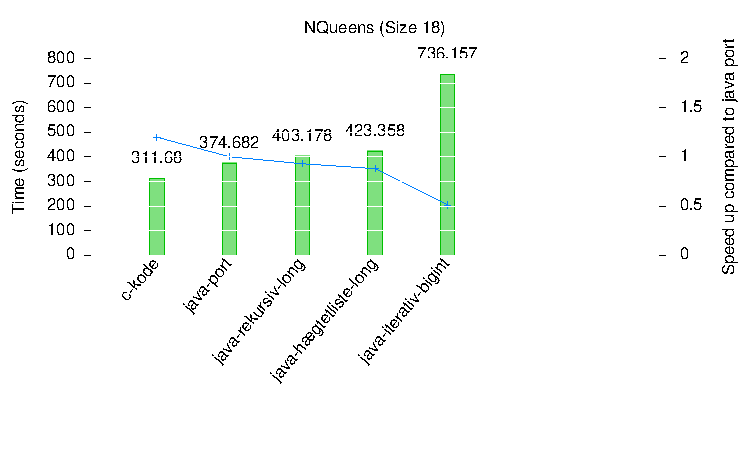
\includegraphics{../benchmarks/lokal2.pdf}   
  
}


	

\section{Ideer til forbedringer}
\frame
{
  \frametitle{Ideer til forbedringer}

  \begin{itemize}
		\item<+-> One-Click
		\begin{itemize}
			\item<+-> Checkpoint() kunne returnere før I/O.
			\item<+-> Webstart fremfor Applets
		\end{itemize}
		\item<+-> NQueen 
		\begin{itemize}
			\item<+-> Undgå serialisering
			\item<+-> Fair opdeling af bræt
		\end{itemize}
				\item<+-> MiG
		\begin{itemize}
			\item<+-> MiG IO - Spildtid mellem hvert job er stor.
		\end{itemize}

  \end{itemize}
}
\end{document}
